\subsubsection{KP04. Manajemen Interaksi Antarpengguna}
\label{kp04}
	\begin{figure}[H]
		\centering
		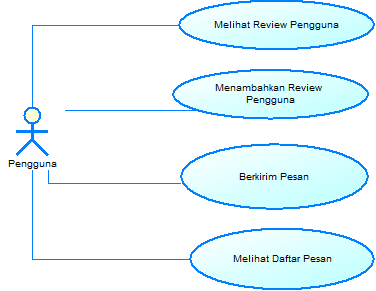
\includegraphics
		[width=\textwidth]
		{images/bab3/usecasediagram/ucd-04.png}
		\caption{Diagram Kasus Penggunaan Manajemen Interaksi Antarpengguna}
		\label{ucd.04}
	\end{figure}
Pada kasus penggunaan ini, pengguna difasilitasi untuk berinteraksi, memberikan \textit{review} / testimoni terhadap pengguna lainnya sesuai dengan keinginan.

	% Melihat review pengguna
	% Melihat review pengguna
	
\begin{table}[H]
	\centering
	\begin{tabular}{|r|p{8cm}|}
		\hline
		\textbf{Kode}                                                    
		& UC-04.01
		\\ \hline
		\textbf{Nama}                                                    
		& \textbf{Melihat \textit{Review} Pengguna} 
		\\ \hline
		
		\textbf{Aktor}  
		& Pengguna 
		\\ \hline
		
		\textbf{Deskripsi}
		& Pengguna ingin melihat \textit{review} pada pengguna tertentu
		\\ \hline
		\textbf{Tipe}                                                    
		& Fungsional 
		\\ \hline
		\textbf{\textit{Precondition}}
		& \textit{Review} pengguna belum ditampilkan
		\\ \hline
		\textbf{\textit{Postcondition}} 
		& \textit{Review} pengguna berhasil ditampilkan
		\\ \hline
		\multicolumn{2}{|c|}
		{\textbf{Alur Kejadian Normal}}                                                                            
		\\ \hline
		\multicolumn{1}{|l|}{} & 
		\begin{enumerate}
			% \item \label{uc0301-show1page}Sistem menampilkan halaman yang berisi form pendaftaran barang
			% \item \label{al-0301-a} Sistem memvalidasi data yang dimasukkan pengguna
			\item Pengguna mengklik \textit{link} profil pengguna
			\item \label{uc0401-a}Sistem menampilkan halaman profil pengguna
			\item Pengguna dapat melihat \textit{review} pengguna di bagian kiri bawah beserta rata-rata \textit{rating} yang diberikan.
		\end{enumerate}
		\\ \hline
		\multicolumn{2}{|c|}{\textbf{Alur Kejadian Alternatif}} \\ \hline
		\multicolumn{1}{|l|}{}                                           
		& -
		\\ \hline
	\end{tabular}
	\caption{Spesifikasi Kasus Penggunaan : Melihat \textit{Review} Pengguna}
	\label{uc04.01}
\end{table}

	
	% Menambahkan Review Pengguna
		% Menambahkan Review Pengguna
	
	
	\begin{table}[H]
		\centering
		\begin{tabular}{|r|p{8cm}|}
			\hline
			\textbf{Kode}                                                    
			& UC-04.02
			\\ \hline
			\textbf{Nama}                                                    
			& \textbf{ Menambahkan Review Pengguna } 
			\\ \hline
			\textbf{Aktor}                                                   
			& Pengguna 
			\\ \hline
			\textbf{Deskripsi}                                               
			& Pengguna ingin menambahkan review dari \textit{transaksi} yang pernah dilakukan.
			\\ \hline
			\textbf{Tipe}
			& Fungsional 
			\\ \hline
			
			\textbf{\textit{Precondition}}
			& Review dari pengguna belum tercatat/tersimpan dalam sistem

			\\ \hline
			
			\textbf{\textit{Postcondition}} 
			& Review dari pengguna berhasil tercatat dalam sistem
			\\ \hline
			
			\multicolumn{2}{|c|}
			{\textbf{Alur Kejadian Normal}}                                                                            
			\\ \hline
			\multicolumn{1}{|l|}{} & 
			\begin{enumerate}
				\item Pengguna mengklik halaman 'Riwayat Transaksi'
				\item Sistem menampilkan halaman Riwayat Transaksi yang pernah dilakukan pengguna
				\item Pengguna mengklik \textit{tab} jenis transaksi yang pernah dilakukan (Beli atau Lelang)
				\item \label{uc0402-show1page}Sistem menampilkan riwayat transaksi sesuai dengan jenis transaksi yang dipilih pengguna
				\item Pengguna mengklik transaksi yang ingin diberikan \textit{review}
				\item \label{al-0402-a}Sistem mengecek apakah \textit{review} sudah pernah diberikan sebelumnya
				\item Sistem menampilkan \textit{modal} berisi \textit{field input} jumlah \textit{rating}
				\item Pengguna mengisi \textit{field} tersebut sesuai jumlah rating yang ingin diberikan
				\item Setelah selesai, pengguna klik 'Next'
				\item Sistem menampilkan \textit{modal} kedua, berisikan \textit{field input} untuk deskripsi \textit{review}
				\item Pengguna mengisikan \textit{field input} sesuai dengan deskripsi yang ingin diberikan
				\item Setelah selesai, pengguna mengklik tombol 'Simpan Review'
				\item \label{al-0402-b}Sistem memvalidasi masukan dari pengguna
				\item Jika tervalidasi, sistem menampilkan modal berisi informasi sukses menyimpan review
				\item Pengguna klik tombol 'Oke'
				\item Sistem menutup \textit{modal} dan kembali ke halaman di poin \cref{uc0402-show1page}
				
				% \item \label{uc0301-show1page}Sistem menampilkan halaman yang berisi form pendaftaran barang
				% \item \label{al-0301-a} Sistem memvalidasi data yang dimasukkan pengguna
			\end{enumerate}
			\\ \hline
			\multicolumn{2}{|c|}{\textbf{Alur Kejadian Alternatif}} \\ \hline
			\multicolumn{1}{|l|}{}                                   \pagebreak        
			& \textbf{Review untuk transaksi yang dipilih sudah pernah diberikan}
			\\ \hline
			\multicolumn{1}{|l|}{}& 
			\begin{itemize}
				\item[\ref{al-0402-a}a.] Sistem mendeteksi bahwa review untuk transaksi tersebut sudah pernah dilakukan
				\item[\ref{al-0402-a}b.] Sistem menampilkan modal berisi informasi bahwa review sudah pernah diberikan, dan \textit{auto-close modal} setelah 4 detik
				\item[\ref{al-0402-a}c.] Sistem menampilkan halaman di poin \cref{uc0402-show1page}
			\end{itemize}
			\\ \hline
			
			\multicolumn{1}{|l|}{}      
			& \textbf{Data masukan pengguna tidak valid}
			\\ \hline
			\multicolumn{1}{|l|}{}& 
			\begin{itemize}
				\item[\ref{al-0402-b}a.] Sistem mendeteksi masukan pengguna tidak valid.
				\item[\ref{al-0402-b}b.] Sistem menampilkan pesan Error berisi \textit{error message}
				\item[\ref{al-0402-b}c.] Sistem menampilkan halaman di poin \cref{uc0402-show1page}
			\end{itemize}
			\\ \hline
		\end{tabular}
		\caption{Spesifikasi Kasus Penggunaan : Memberikan Review Pengguna}
		\label{uc0x.0x-tab}
	\end{table}
	
	% Melaporkan Barang
		% Melaporkan Barang
	
	
	\begin{table}[H]
		\centering
		\begin{tabular}{|r|p{8cm}|}
			\hline
			\textbf{Kode}                                                    
			& UC-04.03
			\\ \hline
			\textbf{Nama}
			
			& \textbf{Melaporkan Barang} 
			\\ \hline
			\textbf{Aktor}                                                   
			& Pengguna 
			\\ \hline
			\textbf{Deskripsi}                                               
			& Pengguna ingin melaporkan barang yang dianggap melanggar aturan/tidak pantas diperjualbelikan
			\\ \hline
			\textbf{Tipe}                                                    
			& Fungsional 
			\\ \hline
			\textbf{\textit{Precondition}}
			& Laporan dari pengguna belum tersimpan dalam sistem
			\\ \hline
			\textbf{\textit{Postcondition}} 
			& Laporan dari pengguna berhasil tersimpan dalam sistem
			\\ \hline
			\multicolumn{2}{|c|}
			{\textbf{Alur Kejadian Normal}}                                                                            
			\\ \hline
			\multicolumn{1}{|l|}{} & 
			\begin{enumerate}
				\item Pengguna mengklik barang yang ingin dilaporkan
				\item \label{uc0403-1page} Sistem menampilkan halaman informasi barang
				\item Pengguna mengklik tombol "Laporkan Barang"
				\item Sistem menampilkan \textit{modal} berisi \textit{input field} laporan
				\item Pengguna mengisi \textit{fields} tersebut sesuai dengan konten laporan yang ingin disampaikan
				\item \label{uc0403-modal}Setelah selesai, pengguna mengklik tombol "Laporkan"
				\item Sistem mengecek dan memvalidasi masukan pengguna
				\item Jika valid, sistem akan menampilkan \textit{modal} Sukses Menyimpan Laporan
				\item Sistem me\textit{redirect} pengguna kembali ke halaman di \ref{uc0403-1page}
				% \item \label{uc0301-show1page}Sistem menampilkan halaman yang berisi form pendaftaran barang
				% \item \label{al-0301-a} Sistem memvalidasi data yang dimasukkan pengguna
			\end{enumerate}
			\\ \hline
			\multicolumn{2}{|c|}{\textbf{Alur Kejadian Alternatif}} \\ \hline
			\multicolumn{1}{|l|}{}      
			& \textbf{Data masukan laporan pengguna tidak valid}
			\\ \hline
			\multicolumn{1}{|l|}{}& 
			\begin{itemize}
				\item[\ref{al-0402-b}a.] Sistem mendeteksi masukan pengguna tidak valid.
				\item[\ref{al-0402-b}c.] Sistem menampilkan kembali modal di poin \ref{uc0403-modal} beserta dengan \textit{error message}
			\end{itemize}
			\\ \hline
		\end{tabular}
		\caption{Spesifikasi Kasus Penggunaan : Melaporkan Barang}
		\label{uc04.03-tab}
	\end{table}
	
	% Berikirim pesan
		% Mengirim pesan
	
	
	\begin{table}[H]
		\centering
		\begin{tabular}{|r|p{8cm}|}
			\hline
			\textbf{Kode}
			& UC-04.04
			\\ \hline
			\textbf{Nama}
			& \textbf{ Mengirim Pesan } 
			\\ \hline
			\textbf{Aktor}    
			& Pengguna 
			\\ \hline
			\textbf{Deskripsi}
			& Pengguna akan mengirimkan pesan kepada pengguna lainnya
			\\ \hline
			\textbf{Tipe}
			& Fungsional 
			\\ \hline
			\textbf{\textit{Precondition}}
			& Pesan yang dikirimkan pengguna belum tersimpan pada sistem
			\\ \hline
			\textbf{\textit{Postcondition}} 
			& Pesan yang dikirimkan pengguna berhasil tersimpan pada sistem
			\\ \hline
			\multicolumn{2}{|c|}
			{\textbf{Alur Kejadian Normal}}
			\\ \hline
			\multicolumn{1}{|l|}{} & 
			\begin{enumerate}
				\item Pengguna mengklik \textit{URL} pengguna tujuan yang ingin dikirimi pesan
				\item Sistem menampilkan halaman profil pengguna tujuan
				\item Pengguna mengklik tombol "Kirim Pesan"
				\item Sistem menampilkan halaman percakapan pengguna terhadap tujuan beserta riwayat percakapan pengguna dengan pengguna tujuan
				\item \label{al-0404-ex} Pengguna memasukkan pesan yang ingin dikirimkan pada \textit{field input} yang disediakan
				\item Setelah selesai, pengguna mengklik tombol 'Kirim'
				\item \label{al-0404-a}Sistem mengirim kepada koneksi soket
				\item Jika proses pengiriman kepada soket berhasil dan tidak ada gangguan, sistem kembali menampilkan halaman pengguna dengan informasi pesan yang sudah terkirim muncul di riwayat percakapan pengguna dengan pengguna tujuan
				
				% \item \label{uc0301-show1page}Sistem menampilkan halaman yang berisi form pendaftaran barang
				% \item \label{al-0301-a} Sistem memvalidasi data yang dimasukkan pengguna
			\end{enumerate}
			\\ \hline
			\multicolumn{2}{|c|}{\textbf{Alur Kejadian Alternatif}} \\ \hline
			\multicolumn{1}{|l|}{}                   
			& \textbf{Terjadi masalah teknis sehingga pesan tidak dapat terkirim}
			\\ \hline
			\multicolumn{1}{|l|}{}& 
			\begin{itemize}
				\item[\ref{al-0404-a}a.] Sistem mendapatkan \textit{exception} dari koneksi soket, bahwa pesan tidak dapat tersimpan
				\item[\ref{al-0404-a}b.] Sistem menampilkan kembali halaman pada poin \ref{al-0404-ex}, dengan \textit{modal} berisikan \textit{error message}
			\end{itemize}
			\\ \hline
		\end{tabular}
		\caption{Spesifikasi Kasus Penggunaan : Mengirimkan Pesan}
		\label{uc04.04-tab}
	\end{table}

	% Melihat daftar pesan
		% Melihat dan membaca pesan
	
	
	\begin{table}[H]
		\centering
		\begin{tabular}{|r|p{8cm}|}
			\hline
			\textbf{Kode}
			& UC-04.05
			\\ \hline
			\textbf{Nama}
			& \textbf{Melihat daftar Pesan} 
			\\ \hline
			\textbf{Aktor}    
			& Pengguna 
			\\ \hline
			\textbf{Deskripsi}
			& Pengguna ingin melihat daftar percakapan/ daftar perpesanan yang pernah dilakukan pengguna
			\\ \hline
			\textbf{Tipe}
			& Fungsional 
			\\ \hline
			\textbf{\textit{Precondition}}
			& Daftar percakapan/ daftar perpesanan belum ditampilkan
			\\ \hline
			\textbf{\textit{Postcondition}} 
			& Daftar percakapan/ daftar perpesanan berhasil ditampilkan
			\\ \hline
			\multicolumn{2}{|c|}
			{\textbf{Alur Kejadian Normal}}
			\\ \hline
			\multicolumn{1}{|l|}{} & 
			\begin{enumerate}
				\item Pengguna mengklik tombol 'Conversations' di \textit{navbar} aplikasi
				\item \label{al-0405-a} Sistem menampilkan halaman daftar percakapan pengguna
				\item Sistem memanggil fungsi AJAX untuk meminta data-data percakapan terakhir pengguna
				\item Balasan dari fungsi AJAX di \textit{load} oleh \textit{browser} untuk selanjutnya di\textit{parse} ke dalam HTML
				\item Sistem menampilkan daftar percakapan pengguna
				\item Pengguna mengklik percakapan yang ingin dilihat/dibaca
				\item Sistem menampilkan detail percakapan pengguna dengan pengguna tujuan
			\end{enumerate}
			\\ \hline
		\end{tabular}
		\caption{Spesifikasi Kasus Penggunaan: Melihat \& Membaca Pesan}
		\label{uc04.05}
	\end{table}
	
	% Menggunakan Kupon
		% Memasukkan kupon
	
	\begin{table}[H]
		\centering
		\begin{tabular}{|r|p{8cm}|}
			\hline
			\textbf{Kode}
			& UC-06.04
			\\ \hline
			\textbf{Nama}
			& \textbf{Memasukkan Kupon pada Transaksi} 
			\\ \hline
			\textbf{Aktor}    
			& Pengguna 
			\\ \hline
			\textbf{Deskripsi}
			& Pengguna ingin menggunakan kupon/voucher yang ia miliki untuk pada sebuah transaksi
			\\ \hline
			\textbf{Tipe}
			& Fungsional 
			\\ \hline
			\textbf{\textit{Precondition}}
			& Pengguna belum berhasil men\textit{submit} kode kupon ke dalam transaksi barang
			\\ \hline
			\textbf{\textit{Postcondition}} 
			& Pengguna berhasil men\textit{submit} kode kupon ke dalam transaksi barang
			\\ \hline
			\multicolumn{2}{|c|}
			{\textbf{Alur Kejadian Normal}}
			\\ \hline
			\multicolumn{1}{|l|}{} & 
			\begin{enumerate}
				\item Pengguna membuka halaman 'Riwayat Transaksi Lelang'
				\item Sistem menampilkan halaman Riwayat Transaksi Lelang pengguna
				\item Pengguna mengklik tombol 'Masukkan Kupon' pada transaksi yang diinginkan
				\item Sistem mengecek permintaan penggunaan kupon
				\item Jika permintaan dapat diverifikasi dan valid, sistem menampilkan \textit{modal} berisi \textit{input field} kupon
				\item Pengguna memasukkan kupon yang ingin dimasukkan, lalu mengklik tombol 'Submit'
				\item Sistem memvalidasi kupon voucher dan status barang
				\item Jika valid, sistem menerapkan penggunaan kupon ke dalam transaksi barang
				\item Sistem lalu menampilkan \textit{modal} yang berisi informasi sukses penggunaan kupon pada transaksi
				% \item \label{uc0301-show1page}Sistem menampilkan halaman yang berisi form pendaftaran barang
				% \item \label{al-0301-a} Sistem memvalidasi data yang dimasukkan pengguna
			\end{enumerate}
			\\ \hline
			\multicolumn{2}{|c|}{\textbf{Alur Kejadian Alternatif}} \\ \hline
			\multicolumn{1}{|l|}{}                   
			& -
			\\ \hline
		\end{tabular}
		\caption{Spesifikasi Kasus Penggunaan : Mendaftarkan Barang Lelang}
		\label{uc04.06}
	\end{table}